\documentclass[border=7mm]{standalone}
\usepackage{fontspec}
% \setmainfont[SmallCapsFeatures={Letters=SmallCaps}]
%      {Linux Libertine O}
% \usepackage{bold-extra}
\usepackage{tikz}
\usetikzlibrary{positioning}

\newcommand{\boxtitle}[1]{\par\large\textbf{\textsf{#1}}\par\vspace{3mm}}
\newcommand{\boxsubtitle}[1]{\vspace{3mm}\par\textbf{\textsf{#1}}\par\vspace{1mm}}
\newcommand{\fonction}[1]{\vspace{1.4mm}\par\textbf{\textit{#1}}\par}

\begin{document}

  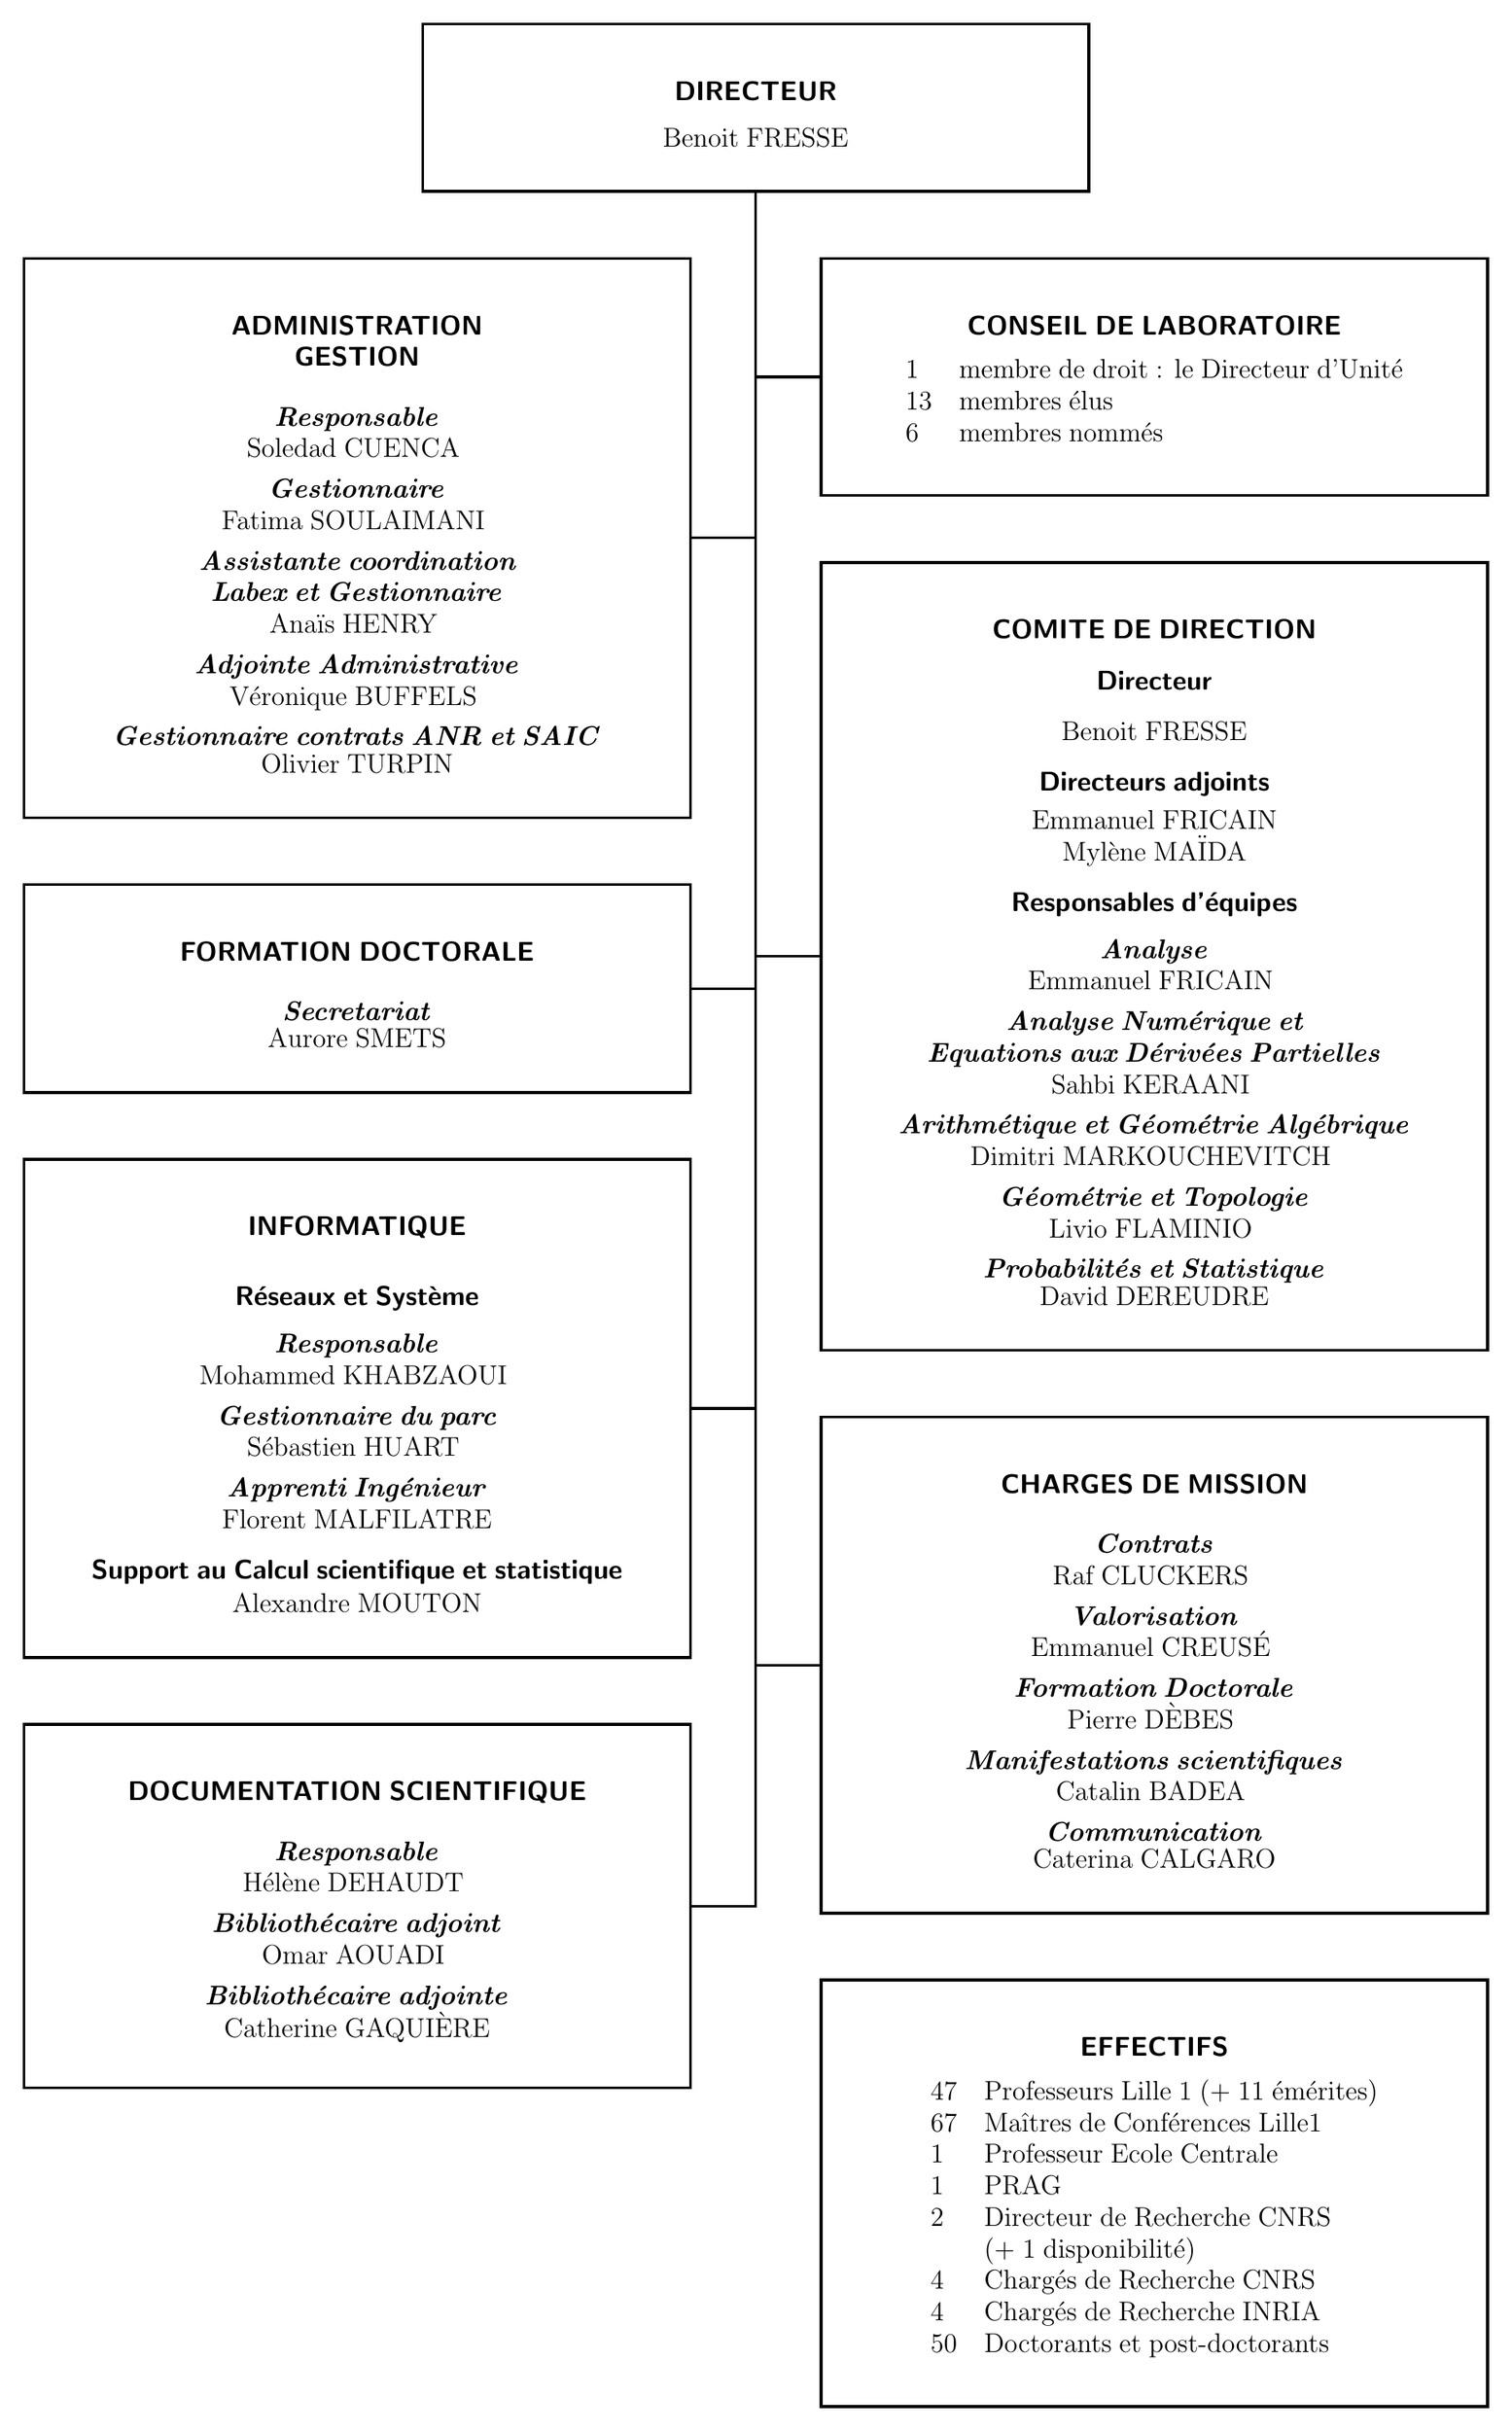
\begin{tikzpicture}[
    every node/.style={
        text width=9cm,
        inner sep= 7mm,
        align=center,
        draw
      },
    very thick
    ]

    % ============= DIRECTEUR ==================

    % -------------------------------
    \node (D) {
      \boxtitle{DIRECTEUR}

      Benoit~FRESSE
    };
    % -------------------------------


    % ============= ADMINISTRATION (GAUCHE) ==================

    % -------------------------------
    \node[below left=of D.south] (AG) {
      \boxtitle{ADMINISTRATION\\GESTION}

      \fonction{Responsable}{Soledad~CUENCA}
      \fonction{Gestionnaire}{Fatima~SOULAIMANI}
      \fonction{Assistante coordination Labex et Gestionnaire}{Anaïs~HENRY}
      \fonction{Adjointe Administrative}{Véronique~BUFFELS}
      \fonction{Gestionnaire contrats ANR et SAIC}{Olivier~TURPIN}
    };
    % -------------------------------

    % -------------------------------
    \node[below=of AG] (FD) {
      \boxtitle{FORMATION DOCTORALE}

      \fonction{Secretariat}{Aurore~SMETS}
    };
    % -------------------------------

    % -------------------------------
    \node[below=of FD] (I) {
      \boxtitle{INFORMATIQUE}

      \boxsubtitle{Réseaux et Système}

      \fonction{Responsable}{Mohammed~KHABZAOUI}
      \fonction{Gestionnaire du parc}{Sébastien~HUART}
      \fonction{Apprenti Ingénieur}{Florent~MALFILATRE}

      \boxsubtitle{Support au Calcul scientifique et statistique}
      Alexandre~MOUTON
    };
    % -------------------------------

    % -------------------------------
    \node[below=of I] (DS) {
      \boxtitle{DOCUMENTATION SCIENTIFIQUE}

      \fonction{Responsable}{Hélène~DEHAUDT}
      \fonction{Bibliothécaire adjoint}{Omar~AOUADI}
      \fonction{Bibliothécaire adjointe}{Catherine~GAQUIÈRE}
    };
    % ============= CONSEILS (DROITE) ==================

    % -------------------------------

    % -------------------------------
    \node[below right=of D.south] (CL) {
      \boxtitle{CONSEIL DE LABORATOIRE}

      \begin{tabular}{ll}
        $1$   & membre de droit : le Directeur d’Unité\\
        $13$  & membres élus\\
        $6$   & membres nommés
      \end{tabular}
    };
    % -------------------------------

    % -------------------------------
    \node[align=center, below=of CL] (CD) {
      \boxtitle{COMITE DE DIRECTION}

      \boxtitle{Directeur}

      Benoit~FRESSE

      \boxsubtitle{Directeurs adjoints}

      Emmanuel~FRICAIN\\Mylène~MAÏDA

      \boxsubtitle{Responsables d’équipes}

      \fonction{Analyse}{Emmanuel~FRICAIN}
      \fonction{Analyse Numérique et\\Equations aux Dérivées Partielles}{Sahbi~KERAANI}
      \fonction{Arithmétique et Géométrie Algébrique}{Dimitri~MARKOUCHEVITCH}
      \fonction{Géométrie et Topologie}{Livio~FLAMINIO}
      \fonction{Probabilités et Statistique}{David~DEREUDRE}
    };
    % -------------------------------

    % -------------------------------
    \node[below=of CD] (CM) {
      \boxtitle{CHARGES DE MISSION}

      \fonction{Contrats}{Raf~CLUCKERS}
      \fonction{Valorisation}{Emmanuel~CREUSÉ}
      \fonction{Formation Doctorale}{Pierre~DÈBES}
      \fonction{Manifestations scientifiques}{Catalin~BADEA}
      \fonction{Communication}{Caterina~CALGARO}
    };
    % -------------------------------

    % -------------------------------
    \node[below=of CM] (E) {
      \boxtitle{EFFECTIFS}

      \begin{tabular}{ll}
        $47$  & Professeurs Lille 1 (+ 11 émérites)\\
        $67$  & Maîtres de Conférences Lille1 \\
        $1$   & Professeur Ecole Centrale\\
        $1$   & PRAG\\
        $2$   & Directeur de Recherche CNRS\\
              & (+ 1 disponibilité)\\
        $4$   & Chargés de Recherche CNRS \\
        $4$   & Chargés de Recherche INRIA\\
        $50$  & Doctorants et post-doctorants
      \end{tabular}
    };

    % ============= LIGNES ==================
    \draw (D) |- (DS)
        (AG) -- (AG-|D)
        (FD) -- (FD-|D)
        (I) -- (I-|D)
        (CL) -- (CL-|D)
        (CD) -- (CD-|D)
        (CM) -- (CM-|D);

  \end{tikzpicture}

\end{document}
